\chapter{Optimization}

Every chapter so far has been, in a quiet way, preparation for this one. We learned
what a derivative is, learned to compute it, learned that it detects where a function
stops rising and starts falling, and learned (through the Mean Value Theorem) why
that detection is trustworthy. All of that machinery was built so that we could
answer a single, very old, very human question: \emph{what is the best you can do?}

Make the box hold the most. Use the least metal. Build the cheapest fence. Run the
shortest distance. Earn the highest profit. These are not artificial textbook
puzzles --- they are the questions that motivated the invention of calculus in the
first place. Fermat was solving max/min problems with a slope-like idea decades
before Newton and Leibniz, and the whole subject of the derivative grew partly out
of the desire to find peaks and valleys without guessing.

This chapter is where calculus earns its keep. The technique is the same one you
already know --- find where the derivative is zero, check the candidates --- but the
hard part, the part nobody warns you about, is everything that happens \emph{before}
you take a derivative: turning a sentence in English (or a picture of a fold-up box)
into a function of one variable, on a definite domain, that you are allowed to
differentiate. That translation is a craft, and most of this chapter is about
learning it well enough that it stops feeling like luck.

\section{What optimization really asks}

Strip away the words and an optimization problem has exactly three ingredients.

\begin{focusbox}
Every applied max/min problem is built from:
\begin{enumerate}
  \item an \textbf{objective} --- the quantity you want to make as large or as small
    as possible (area, volume, cost, distance, time);
  \item one or more \textbf{constraints} --- the conditions tying your choices
    together (a fixed amount of fence, a fixed surface area, a point that must lie on
    a curve);
  \item a \textbf{domain} --- the set of choices that actually make sense (a length
    cannot be negative; a cut cannot be longer than the cardboard).
\end{enumerate}
Your job is to express the objective as a function of \emph{one} variable, find its
extreme value on the domain, and confirm you really found the best.
\end{focusbox}

Why aim for a single variable? We have one tool for finding peaks and valleys: set
the derivative to zero. That tool needs a function of one input. So no matter how many
quantities a problem mentions --- length, width, height, radius, angle --- our first
task is to collapse them down to one, using the constraint to eliminate the rest. The
constraint is not an obstacle; it is the thing that \emph{makes the problem solvable},
because it is what lets us trade many variables for one.

\begin{intuitionbox}
Picture the objective as a landscape and your constraint as a path drawn across it.
Without the constraint you could wander the whole terrain and there might be no
highest point at all. The constraint pins you to a single trail. Now ``the best you
can do'' is just the highest point \emph{on that trail} --- a one-dimensional
question, exactly the kind a derivative can answer. Much of optimization is just
finding the trail.
\end{intuitionbox}

\subsection{A method you can trust}

Here is the recipe we will follow on every single example. Write it on an index
card. The discipline of doing these steps \emph{in order} is what separates a clean
solution from a tangle.

\begin{focusbox}
\textbf{The modeling method for max/min problems.}
\begin{enumerate}
  \item \textbf{Draw a picture} and name the quantities. Introduce letters for the
    things that can vary.
  \item \textbf{Write the objective} --- the thing to be maximized or minimized ---
    as a formula, even if it still has several variables in it.
  \item \textbf{Write the constraint(s)} as equations.
  \item \textbf{Reduce to one variable.} Use the constraint to eliminate every
    variable but one. Now the objective is a function $f$ of a single variable.
  \item \textbf{Find the domain} of that variable --- the interval of values that
    correspond to a real, physical configuration. Note the endpoints.
  \item \textbf{Differentiate and find the critical points}: solve $f'(x)=0$ and note
    where $f'$ fails to exist.
  \item \textbf{Test the candidates.} Compare the values of $f$ at the critical
    points \emph{and} at the endpoints of the domain. Use a first- or second-
    derivative test, or the closed-interval method, to be sure which candidate wins.
  \item \textbf{Answer the question that was asked} --- with units, and check it is
    sane.
\end{enumerate}
\end{focusbox}

Notice that steps 1--5 contain no calculus at all. They are modeling. If you get
those right, step 6 is mechanical. Most ``hard'' optimization problems are really
just modeling problems wearing a calculus disguise.

\begin{whybox}
Why does ``set the derivative to zero'' find the best? Because at an interior point
where $f$ is largest or smallest, the curve must, for that instant, be neither rising
nor falling --- if it were rising, you could nudge a hair to the right and do better;
if falling, a hair to the left. So the tangent there is horizontal: $f'(x)=0$. This
is \emph{Fermat's theorem}, proved cleanly in the chapter on maxima and minima: an
interior extreme of a differentiable function forces a stationary point. Optimization
is just Fermat's theorem applied to a function you had to build yourself. The slope
is the messenger that tells you whether moving helps; where the messenger says
``moving does nothing,'' you may have arrived.
\end{whybox}

\begin{historybox}
The realization that nature and mathematics optimize began in earnest with Pierre de Fermat in 1662. For centuries, optics had been stymied by the law of refraction discovered experimentally by Willebrord Snell in 1621. Fermat proposed a bold physical hypothesis: light traveling between two points does not choose the shortest geometric distance, but the path of \emph{least time} (\emph{Fermat's Principle}). By setting up the total transit time across an optical boundary as a single-variable function of the crossing point $x$,
\[
  T(x) = \frac{\sqrt{a^2+x^2}}{v_1} + \frac{\sqrt{b^2+(d-x)^2}}{v_2},
\]
and setting $T'(x) = 0$ using his method of adequality, Fermat derived Snell's law $\frac{\sin\theta_1}{v_1} = \frac{\sin\theta_2}{v_2}$ from pure mathematics. Nature, it appeared, was an optimizer.

Thirty-four years later, in June 1696, Johann Bernoulli ignited a European competition by posing the celebrated \emph{Brachistochrone problem} in \emph{Acta Eruditorum}: given two points $A$ and $B$ in a vertical plane at different heights, what is the path of a frictionless bead sliding under gravity that minimizes transit time? A straight ramp is the shortest distance, but is it the fastest? 

Five mathematicians solved it: Johann Bernoulli, his brother Jakob Bernoulli, Gottfried Wilhelm Leibniz, Guillaume de l'H\^opital, and Isaac Newton. Newton received the challenge upon returning from a grueling day at the Royal Mint in January 1697, worked through the night, and posted the solution anonymously the next morning. Bernoulli famously recognized the author at once, remarking: ``I recognize the lion by his claw.'' The optimal curve was not a straight line, an arc of a circle, or a parabola---it was a \emph{cycloid}. Bernoulli's challenge broke open the boundary of ordinary optimization: it proved that optimization applies not just to picking a single number $x$, but to discovering an entire unknown function or path, giving birth to the calculus of variations.
\end{historybox}

\section{The closed-interval method: making the answer certain}

Before the examples, let us nail down the one piece of theory that turns a guess into
a guarantee. Setting $f'(x)=0$ tells you where the function \emph{might} peak. It does
not by itself tell you that a peak exists, nor that the candidate you found is the
global best. Two things can go wrong: the maximum might sit at an endpoint of the
domain rather than at a stationary point, or the function might not have a maximum at
all (think of $f(x)=x$ on all of $\R$ --- no biggest value).

The clean fix is the \textbf{Extreme Value Theorem}, which we met in the chapter on
continuity.

\begin{focusbox}
\textbf{Extreme Value Theorem.} If $f$ is continuous on a \emph{closed, bounded}
interval $[a,b]$, then $f$ attains both a maximum and a minimum value somewhere on
$[a,b]$.
\end{focusbox}

This theorem is the optimizer's safety net. As long as your objective is continuous
and your domain is a closed interval $[a,b]$, a best value is \emph{guaranteed to
exist}, and it can only live in one of two kinds of places: at a critical point
inside, or at an endpoint. That gives a finite checklist.

\begin{focusbox}
\textbf{The closed-interval method.} To find the absolute max and min of a continuous
$f$ on $[a,b]$:
\begin{enumerate}
  \item Find all critical numbers in $(a,b)$ (where $f'=0$ or $f'$ does not exist).
  \item Evaluate $f$ at each critical number.
  \item Evaluate $f$ at the two endpoints $a$ and $b$.
  \item The largest of these values is the absolute maximum; the smallest is the
    absolute minimum.
\end{enumerate}
No derivative tests needed --- just compare numbers. The theorem promises the winner
is in your list.
\end{focusbox}

\begin{whybox}
Why is comparing values \emph{enough}? Because the Extreme Value Theorem promises the
maximum is attained \emph{somewhere}. Wherever that somewhere is, it is either an
interior point or an endpoint. If interior, Fermat's theorem says it is a critical
number, so it is in your list. If an endpoint, it is also in your list. There is
nowhere else for it to hide. So you do not need to analyze concavity or signs of
$f'$ at all; you just need to make sure your list of suspects is complete and then
read off the biggest value. The closed-interval method works precisely because the
theorem rules out any fourth possibility.
\end{whybox}

\begin{trapbox}
The closed-interval method requires \emph{three} pieces, and beginners drop one:
\begin{itemize}
  \item \textbf{Continuity}: a jump or a vertical asymptote in the domain breaks the
    guarantee. The function $1/x$ on $[-1,1]$ has no maximum --- it is not continuous
    there.
  \item \textbf{Closed} (endpoints included): on the open interval $(0,1)$ the
    function $f(x)=x$ has no maximum, because it can get arbitrarily close to $1$
    without reaching it.
  \item \textbf{Bounded}: on $[0,\infty)$ the function $f(x)=x$ runs off to infinity.
\end{itemize}
If your domain is not a closed bounded interval, you must argue existence another way
(often by the shape of the graph or a sign analysis of $f'$).
\end{trapbox}

\begin{figure}[H]
\centering
\begin{tikzpicture}
\begin{axis}[
  width=12cm, height=6.2cm,
  axis lines=middle,
  xlabel={$x$}, ylabel={$f(x)$},
  xtick={0.5,4.5}, xticklabels={$a$,$b$},
  ytick=\empty,
  xmin=-0.3, xmax=5.4, ymin=-0.4, ymax=3.6,
  samples=150, domain=0.5:4.5,
  clip=false,
]
\addplot[curveblue, very thick] {1.8 + sin(deg(1.6*(x-0.3)))};
% endpoints
\addplot[only marks, mark=*, mark size=1.7pt, black]
  coordinates {(0.5,2.115) (4.5,2.223)};
% the two interior critical points
\addplot[only marks, mark=*, mark size=1.7pt, tangentred]
  coordinates {(1.282,2.800) (3.245,0.800)};
\node[anchor=south, font=\small] at (axis cs:1.282,2.800) {interior max};
\node[anchor=north, font=\small] at (axis cs:3.245,0.800) {interior min};
\node[anchor=east, font=\small] at (axis cs:0.5,2.115) {endpoint};
\node[anchor=west, font=\small] at (axis cs:4.5,2.223) {endpoint};
\end{axis}
\end{tikzpicture}
\caption{On a closed interval $[a,b]$, the absolute max and min of a continuous
function can only occur at an interior critical point or at an endpoint. The
closed-interval method checks all of them and compares (here both extremes happen to
be interior, with the endpoints landing in between).}
\label{ch17:fig-closed-interval}
\end{figure}

\begin{happeningbox}
When you ``set $f'(x)=0$ and solve,'' what is really happening is a search for
\emph{stationary configurations} --- arrangements where a tiny change in your choice
produces no first-order change in the objective. Think of balancing a ball on a
surface. At a peak, a valley, or a saddle, the ball is momentarily in equilibrium:
the slope is zero in every direction you can move along the constraint. The
derivative is measuring how sensitive your objective is to a small nudge. Setting it
to zero says ``find the spot where I am insensitive to nudges.'' That spot is a
candidate for best, but you still have to check whether it is a peak (max), a valley
(min), or merely a flat shelf --- which is exactly why the second-derivative test and
the closed-interval comparison exist. The vanishing derivative locates equilibria;
the second-order information classifies them.
\end{happeningbox}

\section{Worked example: the open-top box}

Here is the most famous optimization problem in calculus, and deservedly so: it runs
every step of the method on something you can hold in your hands.

\begin{example}[The fold-up box]\label{ch17:ex-box}
You have a square sheet of cardboard $30$ cm on a side. You cut a small square of
side $x$ from each corner, fold up the four flaps, and tape them to make an open-top
box. What size cut $x$ gives the box of \emph{largest volume}?
\end{example}

\textbf{Step 1 --- picture and variables.} Cutting a square of side $x$ from each
corner and folding up leaves a base that is a square of side $30-2x$ (you removed $x$
from each end of every side), and the height of the box is exactly the cut $x$
(Figure~\ref{ch17:fig-box}).

\begin{figure}[H]
\centering
\begin{tikzpicture}
% Left panel: flat sheet with cuts
\begin{scope}[shift={(0,0)}, scale=0.17]
  \fill[structurepurple!8] (0,0) rectangle (30,30);
  \fill[trapred!25] (0,0) rectangle (6,6);
  \fill[trapred!25] (24,0) rectangle (30,6);
  \fill[trapred!25] (0,24) rectangle (6,30);
  \fill[trapred!25] (24,24) rectangle (30,30);
  \fill[sourceblue!20] (6,6) rectangle (24,24);
  \draw[thick] (0,0) rectangle (30,30);
  \draw[dashed, thick, curveblue] (6,6) rectangle (24,24);
  \node[font=\footnotesize] at (15,15) {Base $(30-2x)^2$};
  \node[font=\tiny, trapred!80!black] at (3,3) {cut $x$};
  \node[font=\tiny, trapred!80!black] at (27,3) {cut $x$};
  \node[font=\tiny, trapred!80!black] at (3,27) {cut $x$};
  \node[font=\tiny, trapred!80!black] at (27,27) {cut $x$};
  \draw[<->, >=stealth] (0,-2.5) -- (6,-2.5) node[midway, below, font=\scriptsize] {$x$};
  \draw[<->, >=stealth] (6,-2.5) -- (24,-2.5) node[midway, below, font=\scriptsize] {$30-2x$};
  \draw[<->, >=stealth] (24,-2.5) -- (30,-2.5) node[midway, below, font=\scriptsize] {$x$};
  \draw[<->, >=stealth] (-2.5,0) -- (-2.5,30) node[midway, left, font=\scriptsize] {$30$};
  \node[font=\small, anchor=south] at (15,31.5) {\textbf{Flat Sheet ($30\times 30$)}};
\end{scope}

% Right panel: 3D folded open-top box
\begin{scope}[shift={(7.5,0.6)}]
  % Dimensions: u=(2.6, 0), v=(1.3, 0.9), w=(0, 2.0)
  % Base coordinates:
  \coordinate (A) at (0,0);
  \coordinate (B) at (2.8,0);
  \coordinate (C) at (4.1,1.0);
  \coordinate (D) at (1.3,1.0);
  % Top coordinates:
  \coordinate (A1) at (0,2.0);
  \coordinate (B1) at (2.8,2.0);
  \coordinate (C1) at (4.1,3.0);
  \coordinate (D1) at (1.3,3.0);

  % Shaded inner base and back walls
  \fill[sourceblue!25] (A) -- (B) -- (C) -- (D) -- cycle;
  \fill[sourceblue!12] (D) -- (C) -- (C1) -- (D1) -- cycle;
  \fill[sourceblue!18] (A) -- (D) -- (D1) -- (A1) -- cycle;

  % Hidden edges
  \draw[dashed, gray!70] (A) -- (D) -- (C);
  \draw[dashed, gray!70] (D) -- (D1);

  % Outer visible edges
  \draw[thick, curveblue] (A) -- (B) -- (C);
  \draw[thick, curveblue] (A) -- (A1) (B) -- (B1) (C) -- (C1);
  \draw[thick, curveblue] (A1) -- (B1) -- (C1) -- (D1) -- cycle;

  % Dimension markers
  \draw[<->, >=stealth] (0,-0.35) -- (2.8,-0.35) node[midway, below, font=\scriptsize] {$30-2x$};
  \draw[<->, >=stealth] (2.95,-0.1) -- (4.25,0.9) node[midway, below right, font=\scriptsize] {$30-2x$};
  \draw[<->, >=stealth] (-0.35,0) -- (-0.35,2.0) node[midway, left, font=\scriptsize] {$x$};
  \node[font=\small, anchor=south] at (2.05,3.4) {\textbf{Folded Open-Top Box}};
  \node[font=\footnotesize, curveblue] at (2.05,1.0) {$V = x(30-2x)^2$};
\end{scope}
\end{tikzpicture}
\caption{The fold-up box. Left: Removing square cutouts of side $x$ from each corner
leaves a square base of side $30-2x$. Right: Folding along the dashed lines creates an
open-top box of height $x$, square base $(30-2x)^2$, and volume $V(x)=x(30-2x)^2$.}
\label{ch17:fig-box}
\end{figure}

\textbf{Step 2 --- objective.} The volume is base area times height:
\[
V = (30-2x)^2 \cdot x.
\]
This is already a function of the single variable $x$ --- the geometry handed us the
constraint for free, so there is no separate elimination step here.

\textbf{Step 3 --- domain.} What values of $x$ make a real box? We need $x>0$ (a
genuine cut) and we need the base side $30-2x>0$, i.e.\ $x<15$. At $x=0$ there is no
height; at $x=15$ there is no base. Including those degenerate endpoints (where the
volume is zero) gives the closed interval
\[
0 \le x \le 15.
\]
We deliberately include the endpoints: now the domain is closed and bounded, $V$ is
continuous, and the Extreme Value Theorem guarantees a maximum exists. That is worth
the small fiction of allowing the zero-volume cases.

\textbf{Step 4 --- differentiate.} Expand first to make the derivative painless:
\[
V = x(30-2x)^2 = x(900 - 120x + 4x^2) = 900x - 120x^2 + 4x^3.
\]
Then
\[
V'(x) = 900 - 240x + 12x^2 = 12\,(x^2 - 20x + 75) = 12\,(x-5)(x-15).
\]
\textbf{Step 5 --- critical points.} $V'(x)=0$ at $x=5$ and $x=15$. The point $x=15$
is an endpoint (and gives zero volume), so the only interior critical point is
\[
x = 5.
\]

\textbf{Step 6 --- test.} Use the closed-interval method: evaluate $V$ at the
critical point and both endpoints.
\[
V(0)=0, \qquad V(5) = 5\cdot 20^2 = 5\cdot 400 = 2000, \qquad V(15)=0.
\]
The largest value is $V(5)=2000$, so the maximum volume is $\boxed{2000\text{ cm}^3}$,
achieved by cutting squares of side $\boxed{x=5\text{ cm}}$.

\begin{figure}[H]
\centering
\begin{tikzpicture}
\begin{axis}[
  width=12cm, height=6.4cm,
  axis lines=middle,
  xlabel={cut size $x$ (cm)}, ylabel={volume $V$ (cm$^3$)},
  xtick={0,5,10,15}, ytick={0,1000,2000},
  xmin=-0.4, xmax=16, ymin=-120, ymax=2300,
  samples=150, domain=0:15,
  clip=false,
]
\addplot[curveblue, very thick] {x*(30-2*x)^2};
\addplot[only marks, mark=*, mark size=1.8pt, tangentred] coordinates {(5,2000)};
\draw[dashed, gray] (axis cs:5,0)--(axis cs:5,2000);
\node[anchor=south west, font=\small] at (axis cs:5,2000) {$(5,\,2000)$};
\addplot[only marks, mark=*, mark size=1.6pt, black] coordinates {(0,0) (15,0)};
\end{axis}
\end{tikzpicture}
\caption{Volume of the box as a function of the corner cut $x$. It rises from zero,
peaks at the lone interior critical point $x=5$, and falls back to zero. The peak is
the answer.}
\label{ch17:fig-box-volume}
\end{figure}

\begin{labbox}
Confirm the peak yourself with the second-derivative test. We have $V'(x)=12x^2-240x
+900$, so $V''(x)=24x-240=24(x-10)$. At the critical point, $V''(5)=24(5-10)=-120<0$.
A negative second derivative means concave down means a local maximum --- the curve
is bending downward at $x=5$, so it is a hilltop, not a valley. This agrees with the
closed-interval comparison and gives a second, independent confirmation. Then sketch
the graph from $V(0)=0$, the peak at $(5,2000)$, and $V(15)=0$, and watch it match
Figure~\ref{ch17:fig-box-volume}.
\end{labbox}

\begin{trapbox}
A very common slip on the box problem is to use the side of the base, $30-2x$, as the
height, or to forget that you remove $x$ from \emph{both} ends of each side, writing
the base as $30-x$ instead of $30-2x$. Draw the picture every time. The factor of two
comes straight from the two corners on each edge, and getting it wrong quietly ruins
the whole answer while leaving the algebra looking perfectly healthy.
\end{trapbox}

\section{Worked example: the cheapest can}

Now a problem where the constraint really does extra work, because the objective and
the constraint involve different combinations of the variables.

\begin{example}[The minimal-surface can]\label{ch17:ex-can}
A cylindrical can must hold exactly $355$ cm$^3$ (a standard soda can). What radius
and height minimize the surface area --- that is, use the least metal?
\end{example}

\textbf{Step 1 --- picture and variables.} A cylinder has radius $r$ and height $h$.

\textbf{Step 2 --- objective.} A closed can has a top disk, a bottom disk, and a
wrapped-around side (the lateral surface). The two disks contribute $2\pi r^2$; the
side, if you unroll it, is a rectangle of width $2\pi r$ (the circumference) and
height $h$, contributing $2\pi r h$. So the surface area is
\[
A = 2\pi r^2 + 2\pi r h.
\]
This has \emph{two} variables. We cannot differentiate it yet.

\textbf{Step 3 --- constraint.} The volume is fixed:
\[
\pi r^2 h = 355.
\]

\textbf{Step 4 --- reduce to one variable.} Solve the constraint for the variable
that is easiest to isolate. Here $h$ comes out cleanly:
\[
h = \frac{355}{\pi r^2}.
\]
Substitute into the objective so that $A$ depends on $r$ alone:
\[
A(r) = 2\pi r^2 + 2\pi r\cdot \frac{355}{\pi r^2}
     = 2\pi r^2 + \frac{710}{r}.
\]
This single move --- using the constraint to kill $h$ --- is the heart of the whole
subject. We traded a two-variable problem we cannot solve for a one-variable problem
we can.

\textbf{Step 5 --- domain.} Any positive radius gives a valid can (with $h$ adjusting
to keep the volume right), so the domain is $r>0$, the open interval $(0,\infty)$.
This is \emph{not} a closed bounded interval, so the closed-interval method does not
apply directly --- we will instead use the shape of $A(r)$ to confirm the minimum.
Notice what happens at the ends: as $r\to 0^+$, the term $710/r\to\infty$ (a tall
thin can has a huge side area); as $r\to\infty$, the term $2\pi r^2\to\infty$ (a wide
flat can has huge disks). So $A\to\infty$ at both ends, which already tells us a
minimum sits somewhere in the middle.

\textbf{Step 6 --- differentiate.}
\[
A'(r) = 4\pi r - \frac{710}{r^2}.
\]
Set it to zero:
\[
4\pi r = \frac{710}{r^2}
\quad\Longrightarrow\quad
4\pi r^3 = 710
\quad\Longrightarrow\quad
r^3 = \frac{710}{4\pi} = \frac{177.5}{\pi}.
\]
So
\[
r = \left(\frac{177.5}{\pi}\right)^{1/3} \approx (56.50)^{1/3} \approx 3.837\text{ cm}.
\]
And the height is
\[
h = \frac{355}{\pi r^2} \approx \frac{355}{\pi (3.837)^2}
  \approx \frac{355}{46.25} \approx 7.675\text{ cm}.
\]

\textbf{Step 7 --- confirm it is a minimum.} Two independent checks:
\begin{itemize}
  \item \emph{Second derivative.} $A''(r) = 4\pi + \dfrac{1420}{r^3} > 0$ for every
    $r>0$. The function is concave up everywhere, so the single critical point is a
    minimum --- in fact the \emph{global} minimum, since a function that is concave up
    on all of $(0,\infty)$ can have only one turning point.
  \item \emph{End behavior.} We saw $A\to\infty$ as $r\to0^+$ and as $r\to\infty$,
    with exactly one critical point in between. A continuous function that climbs to
    infinity at both ends and turns around once must turn at a minimum
(Figure~\ref{ch17:fig-can}).
\end{itemize}

\begin{figure}[H]
\centering
\begin{tikzpicture}
\begin{axis}[
  width=12cm, height=6.4cm,
  axis lines=middle,
  xlabel={radius $r$ (cm)}, ylabel={area $A$ (cm$^2$)},
  xtick={1,2,3.837,6}, xticklabels={$1$,$2$,$3.84$,$6$},
  ytick={200,300,400},
  xmin=0, xmax=7, ymin=0, ymax=520,
  samples=200, domain=1.5:6.8,
  clip=true,
]
\addplot[curveblue, very thick] {2*pi*x^2 + 710/x};
\addplot[only marks, mark=*, mark size=1.8pt, tangentred] coordinates {(3.837,277.5)};
\draw[dashed, gray] (axis cs:3.837,0)--(axis cs:3.837,277.5);
\node[anchor=south west, font=\small] at (axis cs:3.837,277.5) {min $\approx(3.84,\,277)$};
\end{axis}
\end{tikzpicture}
\caption{Surface area of a $355$ cm$^3$ can as a function of radius. The two terms
pull in opposite directions: $710/r$ blows up for thin cans, $2\pi r^2$ blows up for
wide cans. The trade-off has a single sweet spot.}
\label{ch17:fig-can}
\end{figure}

\begin{aestheticbox}
Look at the answer: $h \approx 7.675$ and $r \approx 3.837$, so
$h = 2r$. The most efficient closed can is exactly as \emph{tall} as it is
\emph{wide} --- its height equals its diameter, so it fits snugly inside a cube. This
ratio does not depend on the specific number $355$; you get $h=2r$ for \emph{any} fixed volume.
Try it symbolically: minimizing $A=2\pi r^2 + 2V/r$ gives $4\pi r = 2V/r^2$, i.e.
$2\pi r^3 = V = \pi r^2 h$, which simplifies to $h=2r$ no matter what $V$ is. A clean, scale-free
fact sits under the arithmetic. (Real soda cans are taller and
thinner than this --- because the seams and the thicker top cost extra metal the
simple model ignores, and because a hand likes a narrower grip. The math is right; the
model is just simpler than a real can.)
\end{aestheticbox}

\begin{whybox}
Why does substituting the constraint give the right answer, rather than some
distortion? Because the constraint equation $\pi r^2 h = 355$ does not throw any cans
away --- it simply records that for each radius there is exactly one matching height.
The substitution walks along the \emph{curve of all valid cans} in the $(r,h)$ plane,
and $A(r)$ is the genuine surface area of the one valid can with that radius. We are
not approximating; we are restricting attention to the feasible set and reading off
its true area. Minimizing along the trail gives the minimum over all valid cans,
which is exactly what was asked. This is why ``reduce to one variable'' loses
nothing: the eliminated variable was never free --- the constraint had already decided
it.
\end{whybox}

\section{Worked example: the fence with a free side}

A constraint can also be the thing in short supply. This is the classic farmer
problem, and it teaches a lesson about reading the geometry before reaching for
algebra.

\begin{example}[Maximum field, one free side]\label{ch17:ex-fence}
A farmer has $200$ m of fencing and wants to enclose a rectangular field. One side of
the field runs along a straight river and needs no fence. What dimensions enclose the
\emph{largest area}?
\end{example}

\textbf{Step 1 --- picture and variables.} Call the two sides perpendicular to the
river $x$ (there are two of them) and the side parallel to the river $y$ (there is
one of it --- the opposite, river side, is free); see Figure~\ref{ch17:fig-fence}.

\begin{figure}[H]
\centering
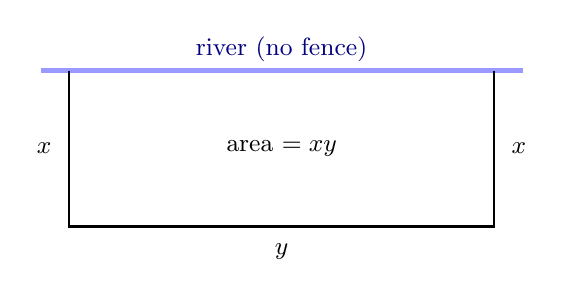
\begin{tikzpicture}[scale=0.9]
% river
\draw[line width=2pt, blue!40] (-0.4,2.2)--(6.4,2.2);
\node[blue!50!black, font=\small] at (3,2.5) {river (no fence)};
% three fenced sides
\draw[thick] (0,2.2)--(0,0)--(6,0)--(6,2.2);
\node[font=\small] at (-0.35,1.1) {$x$};
\node[font=\small] at (6.35,1.1) {$x$};
\node[font=\small] at (3,-0.35) {$y$};
\node[font=\small] at (3,1.1) {area $=xy$};
\end{tikzpicture}
\caption{Three sides are fenced; the river bounds the fourth for free. Fencing used
is $2x+y$.}
\label{ch17:fig-fence}
\end{figure}

\textbf{Step 2 --- objective.} Maximize the area
\[
A = xy.
\]
\textbf{Step 3 --- constraint.} Only three sides use fence, and there are $200$ m of
it:
\[
2x + y = 200.
\]
\textbf{Step 4 --- reduce.} Solve the constraint for $y$: $y = 200 - 2x$. Substitute:
\[
A(x) = x(200-2x) = 200x - 2x^2.
\]
\textbf{Step 5 --- domain.} We need $x>0$ and $y = 200-2x>0$, so $0 < x < 100$;
including the degenerate endpoints (zero area) gives the closed interval $[0,100]$,
and again the Extreme Value Theorem guarantees a maximum.

\textbf{Step 6 --- differentiate.}
\[
A'(x) = 200 - 4x = 0 \quad\Longrightarrow\quad x = 50.
\]
Then $y = 200 - 2(50) = 100$.

\textbf{Step 7 --- test.} Closed-interval comparison:
\[
A(0)=0, \qquad A(50) = 50\cdot 100 = 5000, \qquad A(100)=0.
\]
The maximum area is $\boxed{5000\text{ m}^2}$, with the two short sides $x=50$ m and
the long side $y=100$ m. (The second derivative $A''=-4<0$ confirms concave down, a
maximum.)

\begin{intuitionbox}
Notice the answer splits the fence in a memorable way: the single parallel side $y$
uses $100$ m and the two perpendicular sides together also use $2x=100$ m. The fence
is divided \emph{equally} between the direction along the river and the direction
across it. That balance --- spend half your resource each way --- is the recurring
signature of these rectangle problems, and once you have seen it you can often guess
the answer before differentiating, then use calculus to confirm.
\end{intuitionbox}

\begin{trapbox}
The free side changes the constraint, not the area. A frequent error is to fence all
four sides out of habit, writing $2x+2y=200$, or to optimize the perimeter instead of
the area. Always ask: \emph{which} quantity is fixed (the constraint) and \emph{which}
am I trying to make extreme (the objective)? Here the fence is fixed and the area is
free to grow. Swapping their roles --- maximizing the fence --- is a question with no
answer, and that absurdity is your signal that you mislabeled them.
\end{trapbox}

\section{Worked example: the closest point}

Distance problems hide a small but important computational trick, and they show off
the closed-interval reasoning on a domain that is genuinely infinite.

\begin{example}[Nearest point on a parabola]\label{ch17:ex-distance}
Find the point on the parabola $y = x^2$ that is closest to the point $(0, 2)$.
\end{example}

\textbf{Step 1--2 --- variables and objective.} A point on the parabola is
$(x, x^2)$. Its distance to $(0,2)$ is
\[
D(x) = \sqrt{(x-0)^2 + (x^2 - 2)^2} = \sqrt{x^2 + (x^2-2)^2}.
\]
We want to minimize this.

\textbf{The trick.} Minimizing the distance $D$ is the same as minimizing the
\emph{squared} distance $S = D^2$, because squaring is an increasing function on
$[0,\infty)$ --- wherever $D$ is smallest, $D^2$ is smallest too, and at the same
$x$. So we minimize the square-root-free
\[
S(x) = x^2 + (x^2 - 2)^2,
\]
which is far easier to differentiate. This substitution costs nothing and saves a
chain-rule-through-a-square-root mess.

\begin{whybox}
Why are you allowed to minimize $D^2$ instead of $D$? Because the squaring map
$t\mapsto t^2$ is strictly increasing for $t\ge 0$, and distances are never negative.
A strictly increasing function preserves order: if $D(a) < D(b)$ then $D(a)^2 <
D(b)^2$, and vice versa. So $D$ and $D^2$ rise and fall in lockstep; they have their
minimum at the \emph{same} $x$. The only thing that changes is the messiness of the
derivative. This is a general and very useful move: you may replace your objective by
any strictly increasing function of it (square it, take its log, etc.) without moving
the location of the optimum. Optimizers reach for logs and squares constantly for
exactly this reason.
\end{whybox}

\textbf{Step 3 --- domain.} Any real $x$ gives a point on the parabola, so the domain
is all of $\R = (-\infty, \infty)$. As $\abs{x}\to\infty$ the point on the parabola
shoots off to infinity, so $S\to\infty$ at both ends; a minimum exists in the middle.

\textbf{Step 4 --- differentiate.} Expand:
\[
S(x) = x^2 + x^4 - 4x^2 + 4 = x^4 - 3x^2 + 4.
\]
Then
\[
S'(x) = 4x^3 - 6x = 2x(2x^2 - 3).
\]
\textbf{Step 5 --- critical points.} $S'(x)=0$ gives $x=0$ or $2x^2=3$, i.e.\
$x = \pm\sqrt{3/2} = \pm\sqrt{1.5} \approx \pm 1.225$.

\textbf{Step 6 --- test.} Compare the squared distances at the three critical points:
\[
S(0) = 0 - 0 + 4 = 4,
\]
\[
S\!\left(\pm\sqrt{1.5}\right) = (1.5)^2 - 3(1.5) + 4 = 2.25 - 4.5 + 4 = 1.75.
\]
The smaller value $1.75$ wins, so the closest points are
$\left(\pm\sqrt{1.5},\, 1.5\right)$, at distance $D = \sqrt{1.75} \approx 1.323$
(Figure~\ref{ch17:fig-distance}).

\begin{figure}[H]
\centering
\begin{tikzpicture}
\begin{axis}[
  width=10.5cm, height=7cm,
  axis lines=middle,
  xlabel={$x$}, ylabel={$y$},
  xtick={-1.225,1.225}, xticklabels={$-\sqrt{1.5}$,$\sqrt{1.5}$},
  ytick={1.5,2}, yticklabels={$1.5$,$2$},
  xmin=-2.6, xmax=2.6, ymin=-0.3, ymax=4.2,
  samples=150, domain=-2:2,
  clip=false,
]
\addplot[curveblue, very thick] {x^2};
\addplot[only marks, mark=*, mark size=1.8pt, black] coordinates {(0,2)};
\node[anchor=south west, font=\small] at (axis cs:0,2) {$(0,2)$};
\addplot[only marks, mark=*, mark size=1.8pt, tangentred]
  coordinates {(1.225,1.5) (-1.225,1.5)};
\addplot[dashed, gray] coordinates {(0,2) (1.225,1.5)};
\addplot[dashed, gray] coordinates {(0,2) (-1.225,1.5)};
\end{axis}
\end{tikzpicture}
\caption{The two closest points on $y=x^2$ to the target $(0,2)$, at
$x=\pm\sqrt{1.5}$. The vertex $x=0$ is also a critical point, but there the squared
distance is \emph{largest} among the three candidates (it is a local maximum of $S$,
hence locally the farthest), so it loses the comparison.}
\label{ch17:fig-distance}
\end{figure}

\begin{trapbox}
The vertex $x=0$ is a genuine critical point --- $S'(0)=0$ --- but it is \emph{not} the
answer. In fact $S$ has a local \emph{maximum} there: among the three critical points
the vertex is locally the farthest from $(0,2)$, not the nearest, and the comparison
exposes it. This is exactly why you never stop at ``I found where $S'=0$.'' You must
evaluate $S$ at \emph{all} the critical points and pick the winner. Had you found only
$x=0$ and quit, you would have reported the worst of the three candidates as the best.
The derivative finds suspects; the comparison convicts.
\end{trapbox}

\begin{connectionbox}
A pretty piece of geometry sits behind the algebra. At the true closest point, the
segment from $(0,2)$ to the curve is \emph{perpendicular} to the parabola's tangent
line. To see why: if the connecting segment met the curve at any other
angle, you could slide a little along the curve and get closer, because part of your
motion would be ``toward'' the target. Only when the segment is perpendicular is there
no closer direction to slide. This ``shortest distance is along the normal'' principle
reappears throughout physics (light takes the perpendicular-incidence path, a
stretched string pulls along the normal) and is the geometric soul of the Lagrange
multiplier method you will meet in multivariable calculus. The condition $S'(x)=0$ and
the condition ``segment $\perp$ tangent'' are the same statement in two languages.
\end{connectionbox}

\section{A profit example: optimization beyond geometry}

Optimization is not only about boxes and fences. The same method runs economics,
biology, and machine learning. Here is an example from economics.

\begin{example}[Maximizing profit]\label{ch17:ex-profit}
A workshop can sell $x$ handmade lamps per week. Market research says that to sell $x$
lamps the price per lamp must be $p(x) = 120 - 2x$ dollars (sell more, charge less).
Each lamp costs \$20 to make, plus \$300 in fixed weekly overhead. How many lamps
maximize weekly profit?
\end{example}

\textbf{Objective.} Profit is revenue minus cost. Revenue is price times quantity:
\[
R(x) = x\,p(x) = x(120 - 2x) = 120x - 2x^2.
\]
Cost is overhead plus per-unit cost:
\[
C(x) = 300 + 20x.
\]
So profit is
\[
P(x) = R(x) - C(x) = (120x - 2x^2) - (300 + 20x) = -2x^2 + 100x - 300.
\]

\textbf{Domain.} We need $x\ge 0$, and the price must stay positive: $120-2x>0$ means
$x<60$. So $0 \le x \le 60$ (a closed bounded interval --- the Extreme Value Theorem
applies).

\textbf{Differentiate.}
\[
P'(x) = -4x + 100 = 0 \quad\Longrightarrow\quad x = 25.
\]
\textbf{Test.} $P''(x) = -4 < 0$, concave down everywhere, so $x=25$ is the global
maximum. The profit is
\[
P(25) = -2(625) + 100(25) - 300 = -1250 + 2500 - 300 = 950.
\]
Make $\boxed{25\text{ lamps per week for \$950 profit}}$, at a price of
$p(25) = 120 - 50 = \$70$ each.

\begin{figure}[H]
\centering
\begin{tikzpicture}
\begin{axis}[
  width=12cm, height=6.4cm,
  axis lines=middle,
  xlabel={lamps per week $x$}, ylabel={dollars},
  xtick={0,25,60}, ytick={500,1000,1500},
  xmin=-1, xmax=62, ymin=-1600, ymax=2000,
  samples=120, domain=0:60,
  legend pos=south west, legend style={font=\small, draw=none, fill=none},
  clip=true,
]
\addplot[curveblue, very thick] {120*x - 2*x^2}; \addlegendentry{revenue $R$}
\addplot[quotientorange, very thick] {300 + 20*x}; \addlegendentry{cost $C$}
\addplot[tangentred, very thick, dashed] {-2*x^2 + 100*x - 300}; \addlegendentry{profit $P=R-C$}
\addplot[only marks, mark=*, mark size=1.8pt, black] coordinates {(25,950)};
\draw[dashed, gray] (axis cs:25,-1600)--(axis cs:25,950);
\node[anchor=south west, font=\small] at (axis cs:25,950) {peak profit $(25,\,950)$};
\end{axis}
\end{tikzpicture}
\caption{Revenue, cost, and profit for the lamp workshop. Profit peaks where its slope
is zero --- equivalently, where the revenue and cost curves are momentarily climbing at
the \emph{same} rate, i.e.\ marginal revenue equals marginal cost (at $x=25$).}
\label{ch17:fig-profit}
\end{figure}

\begin{applicationbox}
Economists recognize the condition $P'(x)=0$ as the famous rule \emph{marginal
revenue equals marginal cost}. Watch: $P'=R'-C'$, so $P'=0$ means $R'(x)=C'(x)$. The
derivative $R'$ is the extra revenue from selling one more unit (marginal revenue) and
$C'$ is the extra cost of making one more unit (marginal cost). The rule says: keep
producing as long as the next unit brings in more than it costs, and stop the instant
they balance (Figure~\ref{ch17:fig-profit}). Past that point each extra lamp costs more
than it earns and profit falls. The entire theory of the profit-maximizing firm is this one derivative set to
zero --- the same Fermat condition as the cardboard box, in the language of money.
\end{applicationbox}

\begin{applicationbox}
The same skeleton drives modern machine learning. Training a model means choosing
parameters to \emph{minimize} a loss function --- the objective is the error, the
variables are the millions of weights, and ``learning'' is optimization. There is no
clean constraint to substitute and no formula for the answer, so instead of solving
$\nabla(\text{loss})=0$ exactly, the computer rolls downhill: it repeatedly steps in
the direction the gradient says decreases the loss fastest (gradient descent). But the
target is unchanged from this chapter --- a place where the derivative vanishes, a
stationary point of the objective. Every example here is a hand-solvable instance of
what a neural network does numerically a billion times over.
\end{applicationbox}

\section{When the candidate is not the answer: pitfalls and checks}

The single most common way to lose points --- and to be flatly wrong in real life ---
is to find a critical point and \emph{assume} it is the extreme you want. It might be
a minimum when you wanted a maximum. It might be a local extreme beaten by an
endpoint. It might be a saddle-like inflection that is neither. Here is how to make
sure.

\begin{focusbox}
\textbf{Three ways to confirm you found the right extreme.}
\begin{enumerate}
  \item \textbf{Closed-interval method} (best when the domain is a closed bounded
    interval): evaluate the objective at every critical point and both endpoints,
    then read off the largest/smallest. The Extreme Value Theorem guarantees the
    winner is in your list. No further argument needed.
  \item \textbf{First-derivative test} (works on any interval): check the sign of
    $f'$ just left and just right of the critical point. Sign change $+\to-$ means a
    local max; $-\to+$ means a local min; no change means neither.
  \item \textbf{Second-derivative test} (quick when $f''$ is easy): at a critical
    point, $f''<0$ means local max (concave down), $f''>0$ means local min (concave
    up). If $f''=0$ the test is silent --- fall back to method 1 or 2.
\end{enumerate}
For an \emph{open} or \emph{unbounded} domain, also check the behavior at the open
ends (limits as $x$ approaches the boundary or $\pm\infty$) to be sure a max or min
exists at all.
\end{focusbox}

\begin{trapbox}
\textbf{The endpoint that wins.} Suppose you must minimize $f(x) = x^3 - 3x$ on
$[0, 3]$. The critical points solve $f'(x) = 3x^2 - 3 = 0$, giving $x=\pm 1$; only
$x=1$ is in the domain, and there $f(1) = 1 - 3 = -2$. If you stopped there you would
report the minimum as $-2$ --- and you would be right. But if instead the problem asked
for the \emph{maximum} on $[0,3]$, the critical point $x=1$ is a local \emph{minimum},
not a maximum at all. The maximum lives at the endpoint: $f(3) = 27 - 9 = 18$ versus
$f(0)=0$. The lesson: the interesting answer is sometimes at the edge of the domain,
where the derivative never vanishes (Figure~\ref{ch17:fig-endpoint}).
\emph{Always check the endpoints.}
\end{trapbox}

\begin{figure}[H]
\centering
\begin{tikzpicture}
\begin{axis}[
  width=11cm, height=6cm,
  axis lines=middle,
  xlabel={$x$}, ylabel={$f(x)$},
  xtick={0,1,3}, ytick={-2,18},
  xmin=-0.4, xmax=3.4, ymin=-4, ymax=20,
  samples=150, domain=0:3,
  clip=false,
]
\addplot[curveblue, very thick] {x^3 - 3*x};
\addplot[only marks, mark=*, mark size=1.7pt, tangentred] coordinates {(1,-2)};
\addplot[only marks, mark=*, mark size=1.7pt, black] coordinates {(0,0) (3,18)};
\node[anchor=north, font=\small] at (axis cs:1,-2) {crit.\ pt (a min)};
\node[anchor=south east, font=\small] at (axis cs:3,18) {max at endpoint};
\end{axis}
\end{tikzpicture}
\caption{$f(x)=x^3-3x$ on $[0,3]$. The only interior critical point is a
\emph{minimum}; the maximum hides at the right endpoint. Find the critical points,
but let the comparison --- not your hopes --- pick the winner.}
\label{ch17:fig-endpoint}
\end{figure}

\begin{walkbox}
Take a walk and think about \emph{existence} versus \emph{location}. The derivative
is a tool for \emph{location}: it points at where an extreme could be. But it says
nothing about whether an extreme \emph{exists}. What guarantees existence? On a closed
bounded interval, continuity does (the Extreme Value Theorem). On an open or infinite
domain you need something else --- the function running off to infinity at both ends,
say, or a single turning point. Ask yourself: for each worked example in this chapter,
\emph{what} guaranteed the answer existed before I trusted the critical point? You
will find the closed-interval cases leaned on the theorem, while the can and the
distance problems leaned on $\to\infty$ end-behavior. Existence and location are two
separate questions, and a complete solution answers both.
\end{walkbox}

\begin{happeningbox}
When a problem has no maximum, the symptom is usually that the objective improves
forever as you slide toward a boundary the domain does not include. ``Find the
rectangle of largest area with perimeter at most $100$'' has an answer; ``find the
rectangle of largest area'' (no constraint) does not --- you can always make a bigger
one. The constraint is what bounds the feasible set and lets a best exist. So when a
real optimization has no solution, the deepest fix is rarely more calculus; it is
finding the missing constraint --- the budget, the material limit, the physical wall ---
that the problem forgot to state. Calculus locates the optimum; modeling guarantees
there is one to locate.
\end{happeningbox}

\section{A fully general template, worked symbolically}

To cement that the method is one method, let us do the fence problem's cousin
\emph{with letters instead of numbers}, so you can see the structure stand on its own.

\begin{example}[Largest rectangle inscribed under a parabola]\label{ch17:ex-inscribed}
A rectangle sits with its base on the $x$-axis and its top two corners on the
downward parabola $y = c - x^2$ (with $c>0$), symmetric about the $y$-axis. What width
makes its area largest?
\end{example}

\textbf{Variables.} By symmetry the top corners are at $(\pm x, c - x^2)$ for some
$x>0$. The rectangle then has width $2x$ and height $c - x^2$.

\textbf{Objective.}
\[
A(x) = (\text{width})(\text{height}) = 2x\,(c - x^2) = 2cx - 2x^3.
\]
\textbf{Domain.} We need the top corners above the axis, $c - x^2 \ge 0$, so
$0 \le x \le \sqrt{c}$ --- a closed bounded interval.

\textbf{Differentiate.}
\[
A'(x) = 2c - 6x^2 = 0 \quad\Longrightarrow\quad x^2 = \frac{c}{3}
\quad\Longrightarrow\quad x = \sqrt{c/3}.
\]
\textbf{Test.} The endpoints give $A(0)=0$ and $A(\sqrt c)=0$, while the critical
point gives a positive value, so the critical point is the maximum. (Or use
$A''(x)=-12x<0$ for $x>0$.) The maximal area is
\[
A\!\left(\sqrt{c/3}\right) = 2\sqrt{\tfrac{c}{3}}\left(c - \tfrac{c}{3}\right)
= 2\sqrt{\tfrac{c}{3}}\cdot \tfrac{2c}{3}
= \frac{4c}{3}\sqrt{\frac{c}{3}}.
\]

\begin{figure}[H]
\centering
\begin{tikzpicture}
\begin{axis}[
  width=11.5cm, height=6.4cm,
  axis lines=middle,
  xlabel={$x$}, ylabel={$y$},
  xtick={-1.732, -1, 0, 1, 1.732},
  xticklabels={$-\sqrt{c}$, $-\sqrt{\frac{c}{3}}$, $0$, $\sqrt{\frac{c}{3}}$, $\sqrt{c}$},
  ytick={2, 3},
  yticklabels={$\frac{2}{3}c$, $c$},
  xmin=-2.2, xmax=2.2, ymin=-0.4, ymax=3.5,
  samples=120, domain=-1.85:1.85,
  clip=false,
  title style={font=\small},
]
% Parabola with c=3: y = 3 - x^2
\addplot[curveblue, very thick] {3 - x^2};
% Inscribed rectangle for c=3: x in [-1, 1], y in [0, 2]
\fill[sourceblue!25, draw=structurepurple, thick] (axis cs:-1,0) rectangle (axis cs:1,2);
\addplot[only marks, mark=*, mark size=1.8pt, tangentred] coordinates {(-1,2) (1,2)};
\addplot[only marks, mark=*, mark size=1.8pt, curveblue] coordinates {(0,3)};
\draw[dashed, gray] (axis cs:-2,2) -- (axis cs:2,2);
\node[anchor=south west, tangentred, font=\footnotesize] at (axis cs:1,2.05) {$\left(\sqrt{\frac{c}{3}},\,\frac{2}{3}c\right)$};
\node[anchor=center, font=\footnotesize, structurepurple] at (axis cs:0,1.0) {Area $= \frac{4c}{3}\sqrt{\frac{c}{3}}$};
\node[anchor=south, curveblue, font=\small] at (axis cs:0,3.05) {Peak $(0,c)$};
\end{axis}
\end{tikzpicture}
\caption{The optimal rectangle inscribed under the parabola $y = c - x^2$ (shown for
$c=3$). The upper corners meet the curve at $x = \pm\sqrt{c/3}$, fixing the optimal
height at exactly two-thirds of the parabola's maximum height: $y = \frac{2}{3}c$.}
\label{ch17:fig-inscribed}
\end{figure}

\begin{aestheticbox}
The optimal height is $c - x^2 = c - \tfrac{c}{3} = \tfrac{2c}{3}$ --- exactly
\emph{two-thirds} of the parabola's peak height $c$, no matter what $c$ is. The best
rectangle always reaches two-thirds of the way up. Solving the problem once, with a
letter, reveals a clean ratio that a hundred numerical versions would only hint at.
This is the payoff of the symbolic approach: numbers give answers, but letters give
\emph{laws}.
\end{aestheticbox}

\section{Summary: the shape of every solution}

\begin{focusbox}
\textbf{What to carry away.}
\begin{itemize}
  \item Optimization $=$ objective $+$ constraint $+$ domain. The first and hardest
    job is \emph{modeling}: turning words and pictures into a one-variable function
    on a definite domain.
  \item The constraint is your friend: it is what lets you eliminate variables and
    reach a single-variable function the derivative can handle.
  \item Critical points (where $f'=0$ or $f'$ is undefined) are \emph{candidates},
    not answers. Endpoints are candidates too.
  \item On a closed bounded interval, the Extreme Value Theorem guarantees a best
    exists, and the closed-interval method finds it by comparing values --- no
    derivative test required.
  \item On open or infinite domains, you must separately argue that an extreme exists
    (end behavior, concavity, or a single turning point).
  \item Confirm with the closed-interval comparison, the first-derivative test, or
    the second-derivative test --- and always sanity-check units and plausibility.
  \item The very same method --- Fermat's vanishing slope --- runs geometry, physics,
    economics, and machine learning. It is the most widely used idea in all of
    calculus.
\end{itemize}
\end{focusbox}

\subsection{Extrema in Nature and the Multivariable Frontier}
\label{ch17:what-unlocked}

\begin{connectionbox}
Optimization gave calculus its primary mandate in the physical and commercial world. Through Fermat's stationarity principle and the closed-interval method:
\begin{itemize}
  \item \emph{Physical variational principles}: Light rays, gravitational orbits, and hanging chains follow trajectories that extremize fundamental physical quantities like time and action.
  \item \emph{Engineering design}: Structural envelopes, beverage containers, and mechanical linkages can be designed to minimize material consumption, minimize drag, or maximize structural rigidity under physical constraints.
  \item \emph{Economic equilibrium}: Monopolists and competitive firms determine profit-maximizing production quantities by equating marginal revenue to marginal cost ($R'(q) = C'(q)$).
\end{itemize}

Yet these methods are fundamentally restricted to \emph{single-variable} problems (or two-variable problems that can be collapsed to one variable via algebraic substitution). In the real world, optimization rarely presents itself so neatly:
\begin{itemize}
  \item In practical engineering and machine learning, objectives depend on dozens, thousands, or billions of variables.
  \item Constraints are frequently non-linear or implicitly coupled equations $g_1(x,y,z)=0, \dots, g_k(x,y,z)=0$ that cannot be solved algebraically for one variable in terms of the others.
  \item Solving single-variable equations via substitution often destroys natural physical symmetries and introduces artificial coordinate singularities.
\end{itemize}

To break through this bottleneck, we must advance to multivariable calculus. In Chapter~33 (\emph{The Gradient, Directional Derivatives, and the Multivariable Chain Rule}), we encounter the geometric masterpiece of constrained optimization: \emph{Lagrange multipliers}. Instead of algebraically eliminating variables, we optimize an objective $f(\vec{x})$ subject to $g(\vec{x})=c$ by matching their normal vectors: $\grad f = \lambda \grad g$.
\end{connectionbox}

\section{Exercises}

\begin{exercise}[Open-top box, rectangular sheet]
A box with an open top is made from a $16\text{ cm}\times 10\text{ cm}$ rectangle of
cardboard by cutting equal squares of side $x$ from the corners and folding up the
sides. (a) Write the volume $V(x)$. (b) State the domain of $x$. (c) Find the cut $x$
that maximizes the volume, and give the maximum volume. (d) Confirm with the
second-derivative test.
\end{exercise}

\begin{exercise}[The cheapest open-top can]
An \emph{open-top} cylindrical can (no lid) must hold $1000\text{ cm}^3$. (a) Write
the surface area as a function of the radius $r$ alone. (b) Find the radius and height
that minimize the metal used. (c) Show that for the open-top can the optimal height
equals the radius, $h=r$ --- contrast this with $h=2r$ for the closed can, and explain
in words why losing the lid makes the optimal can relatively shorter.
\end{exercise}

\begin{exercise}[Fence with a divider]
A farmer has $240$ m of fencing to build a rectangular pen \emph{and} an internal
fence parallel to one side that splits the pen into two equal halves. (a) If $x$ is
the length of the divided direction (so three segments of length $x$ are needed) and
$y$ the other, write the constraint and the area objective. (b) Find the dimensions of
maximum total area. (c) How does the answer compare to the no-divider case?
\end{exercise}

\begin{exercise}[Closest point on a line]
Find the point on the line $y = 2x + 1$ closest to the origin. (a) Minimize the
\emph{squared} distance and explain why that is legitimate. (b) Verify that the
segment from the origin to your point is perpendicular to the line, and explain
geometrically why it must be.
\end{exercise}

\begin{exercise}[Norman window]
A ``Norman window'' is a rectangle topped by a semicircle whose diameter equals the
rectangle's width. The total perimeter is fixed at $P$ meters. Find the dimensions
admitting the most light (i.e.\ the largest area). Express the optimal rectangle width
in terms of $P$.
\end{exercise}

\begin{exercise}[Maximum-area triangle]
Among all right triangles with legs summing to a fixed length $L$ (so leg$_1+$leg$_2
= L$), find the one with the largest area. What is special about its shape? Prove your
answer is a maximum, not a minimum.
\end{exercise}

\begin{exercise}[An endpoint maximum]
Find the absolute maximum and absolute minimum of $f(x) = x^3 - 6x^2 + 9x + 2$ on the
closed interval $[0,5]$ using the closed-interval method. Identify which extreme
occurs at a critical point and which (if any) at an endpoint.
\end{exercise}

\begin{exercise}[Time, not distance: the lifeguard problem]
A lifeguard at point $A$ on a straight beach must reach a swimmer at point $B$ in the
water. She runs along the sand at speed $v_1$ and swims at the slower speed $v_2 <
v_1$. Setting up coordinates so the shoreline is the $x$-axis, $A=(0,a)$ with $a>0$, and
$B=(d, -h)$ with $h>0$, she enters the water at the point $(x,0)$. (a) Write the total
travel \emph{time} $T(x)$. (b) Show that $T'(x)=0$ leads to the condition
$\dfrac{\sin\theta_1}{\sin\theta_2} = \dfrac{v_1}{v_2}$, where $\theta_1,\theta_2$ are
the angles the running and swimming paths make with the line perpendicular to the
shore. (This is \emph{Snell's law of refraction} --- light minimizes travel time the
same way.)
\end{exercise}

\begin{exercise}[Why $h=2r$, in general]
For a closed cylindrical can of fixed volume $V$, minimize the surface area
\emph{symbolically} (keep $V$ as a letter) and prove that the optimal can always
satisfies $h = 2r$, independent of $V$. Then prove the critical point is a minimum
using the second derivative.
\end{exercise}

\begin{exercise}[Conceptual: existence]
Give an example of a continuous function on an \emph{open} interval that has a
critical point which is not its absolute maximum, and explain why the closed-interval
method cannot be applied. Then state precisely what additional information would let
you conclude that an absolute maximum exists.
\end{exercise}

\begin{exercise}[Proof: substitution preserves the optimum]
Suppose you minimize $f(x)$ over a domain $D$, and $g$ is a strictly increasing
function defined on the range of $f$. Prove that $f$ and $g\circ f$ attain their
minimum at exactly the same points of $D$. (This is the theorem that justifies
minimizing $D^2$ instead of $D$, or minimizing a log-likelihood instead of a
likelihood.)
\end{exercise}
